\section{Propuesta de solución}
\label{sec:propuesta}

Para abordar la extracción automática del total en facturas, se ha desarrollado un pipeline modular que combina OCR, preprocesamiento de texto y un clasificador de candidatos numéricos. El desarrollo se ha organizado en tres fases experimentales sucesivas, cada una construyendo sobre los hallazgos de la anterior.

\subsection{Fase 1: Comparativa de modelos de extracción}

Se implementaron y evaluaron ocho modelos de extracción sobre los mismos datos de entrenamiento (779 muestras CORD) y test (95 muestras):

\begin{itemize}
    \item \textbf{Basados en reglas:} Regex Keyword (busca ``total'' + número adyacente) y Regex Max Filtrado (mayor número filtrando contextos negativos).
    \item \textbf{ML clásico:} Candidate Random Forest, Candidate Gradient Boosting y Candidate SVM, que clasifican candidatos numéricos mediante 12 características (posición relativa, magnitud, proximidad a keywords, contexto positivo/negativo, etc.).
    \item \textbf{NLP clásico:} TF-IDF + Logistic Regression con 3000 features y 1-2 gramas.
    \item \textbf{Deep Learning:} DistilBERT Reranker (clasificador binario fine-tuned) y T5 Seq2Seq (generación directa del total).
\end{itemize}

\begin{figure}[t]
    \centering
    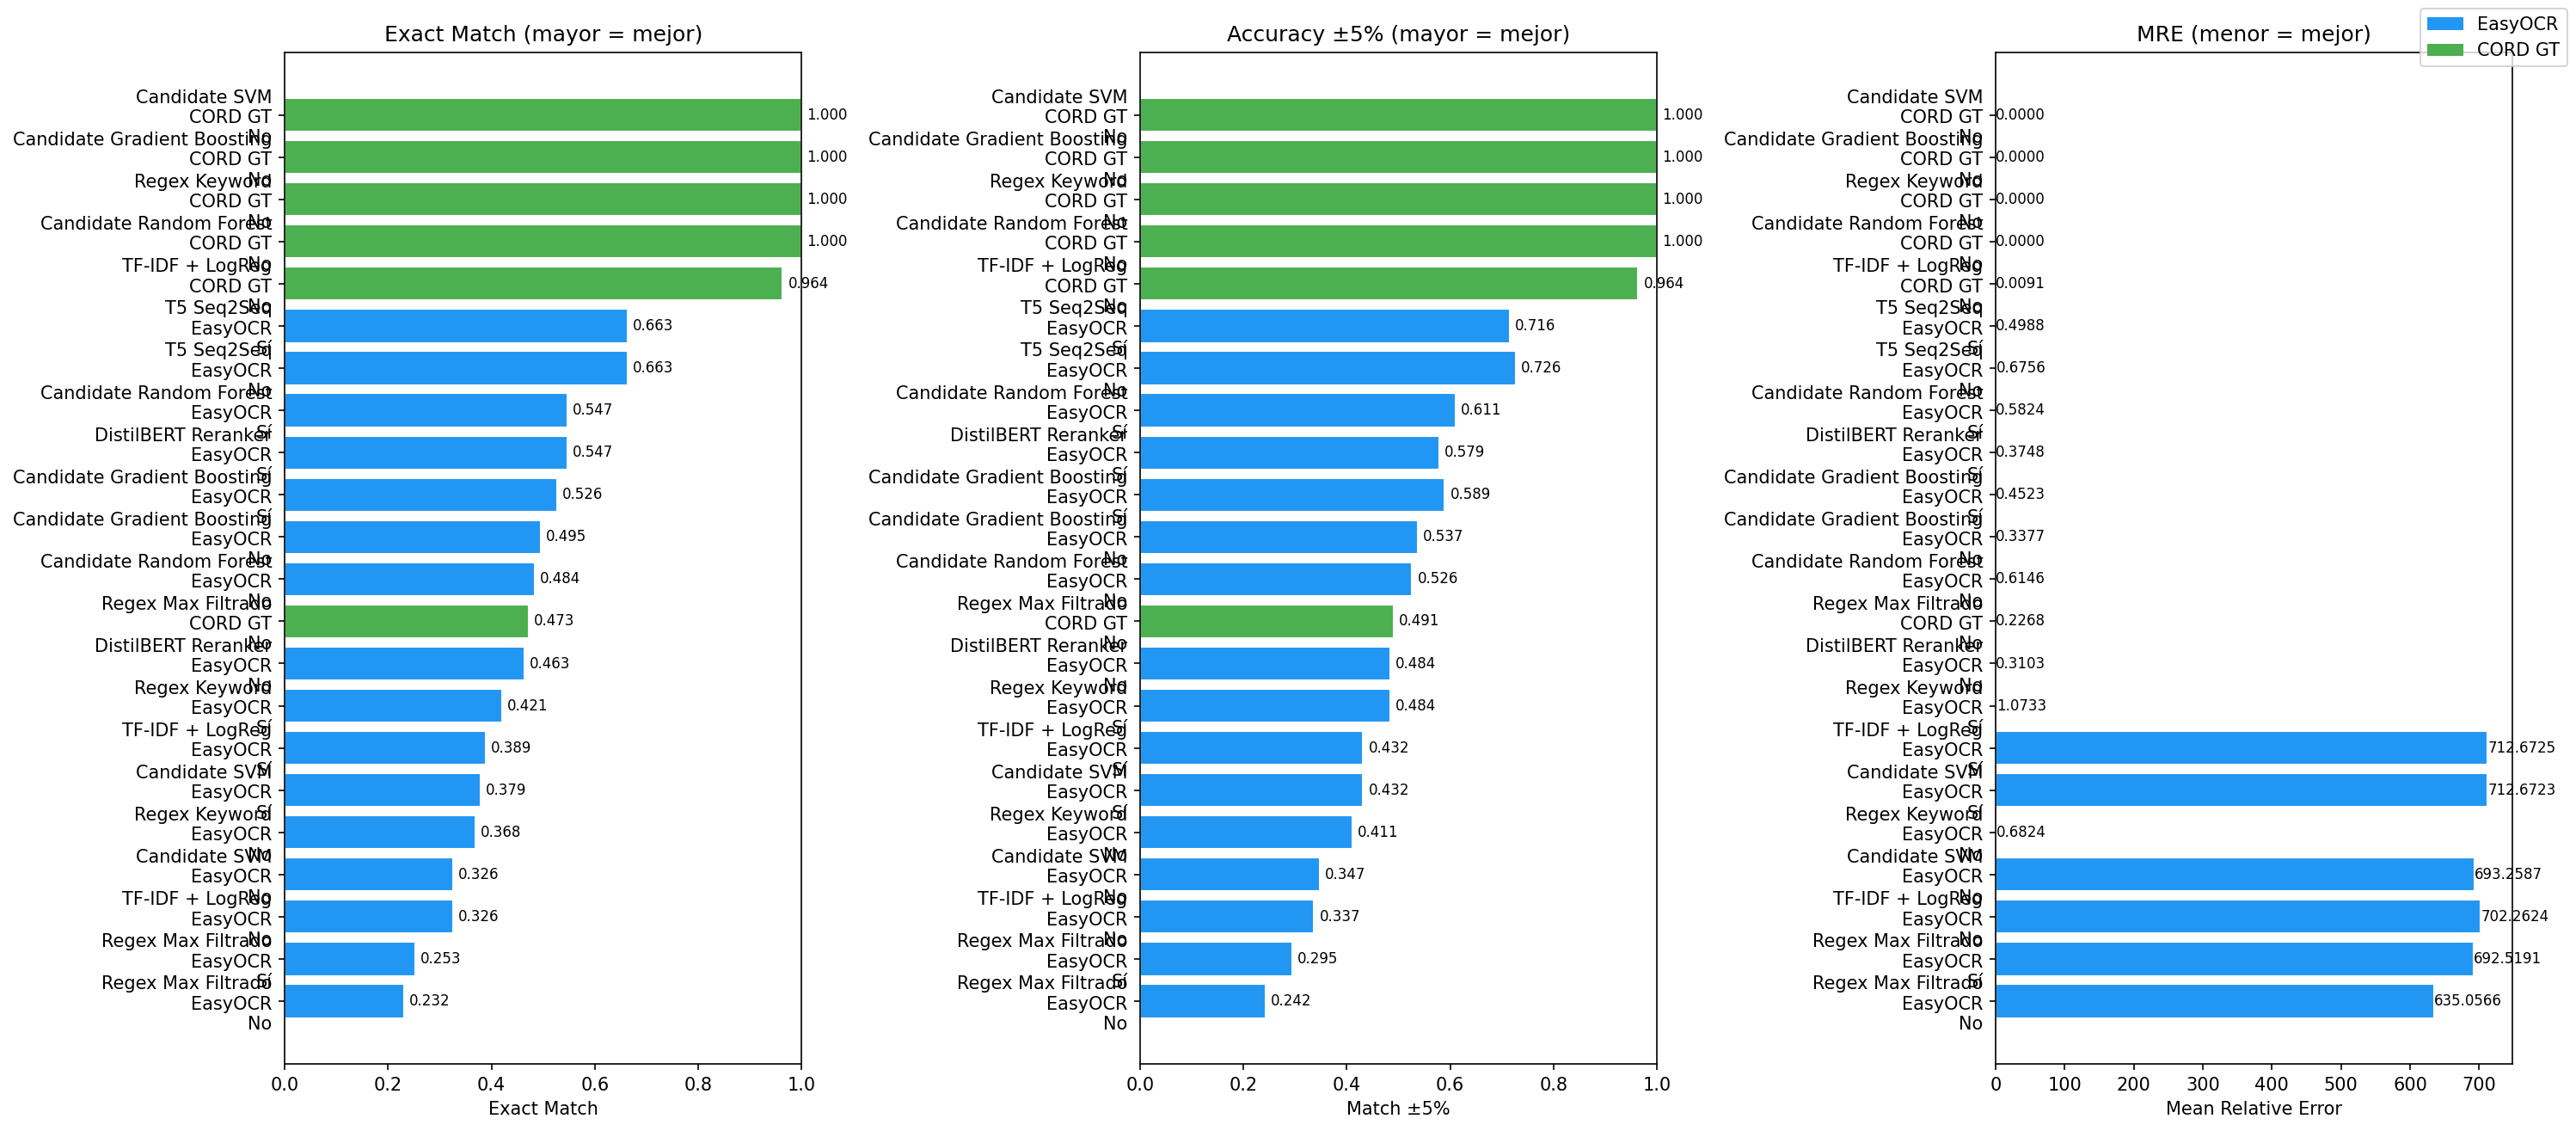
\includegraphics[width=\textwidth]{figures/comparativa_general.png}
    \caption{Comparativa general de los 8 modelos evaluados con EasyOCR: Exact Match, Match $\pm$5\% y MRE}
    \label{fig:comparativa_general}
\end{figure}

Como se observa en la Figura~\ref{fig:comparativa_general}, T5 obtuvo la mayor precisión (66,3\% Exact Match) pero con un coste inviable para móvil: 900~MB y 14~s por predicción. DistilBERT no justificó sus 250~MB al igualar a Random Forest. \textbf{Gradient Boosting} ofreció el mejor equilibrio calidad/coste: 52,6\% Exact Match, 0,18~s de predicción y $\sim$2~MB de modelo.

Un hallazgo clave fue que todos los modelos alcanzan el 100\% de precisión con texto limpio (\textit{ground truth}), demostrando que \textbf{el cuello de botella es la calidad del OCR}, no el modelo de extracción.

\begin{figure}[t]
    \centering
    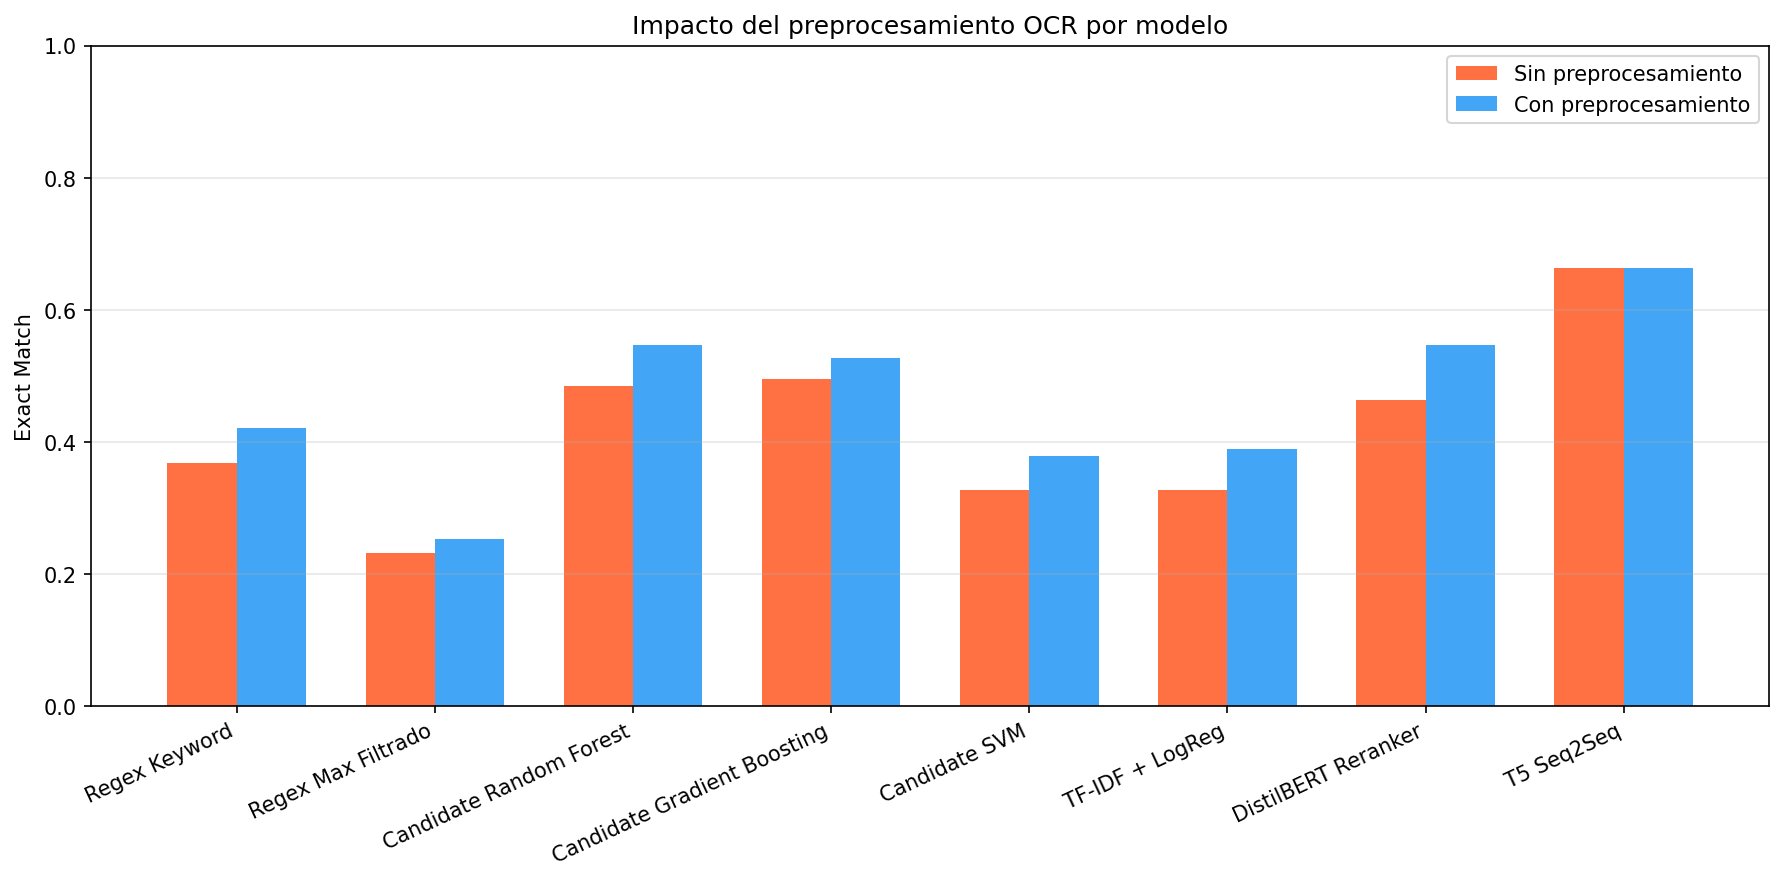
\includegraphics[width=0.8\textwidth]{figures/impacto_preprocesamiento.png}
    \caption{Impacto del preprocesamiento de texto OCR por modelo: la corrección de errores mejora todos los modelos entre 4 y 8 puntos porcentuales}
    \label{fig:impacto_preprocesamiento}
\end{figure}

El preprocesamiento de texto OCR (Figura~\ref{fig:impacto_preprocesamiento}) demostró mejorar consistentemente todos los modelos entre 4 y 8 puntos porcentuales. Este paso corrige errores típicos del OCR: \texttt{O}$\rightarrow$\texttt{0}, \texttt{l}$\rightarrow$\texttt{1}, \texttt{D}$\rightarrow$\texttt{0} cuando están adyacentes a dígitos, además de eliminar caracteres basura y normalizar espacios.

\subsection{Fase 2: Pipeline móvil híbrido}

Se propuso un pipeline de dos pasos para dispositivos móviles: primero Regex Keyword (0,01~ms) y, si falla, Gradient Boosting como fallback (2~ms).

\begin{figure}[t]
    \centering
    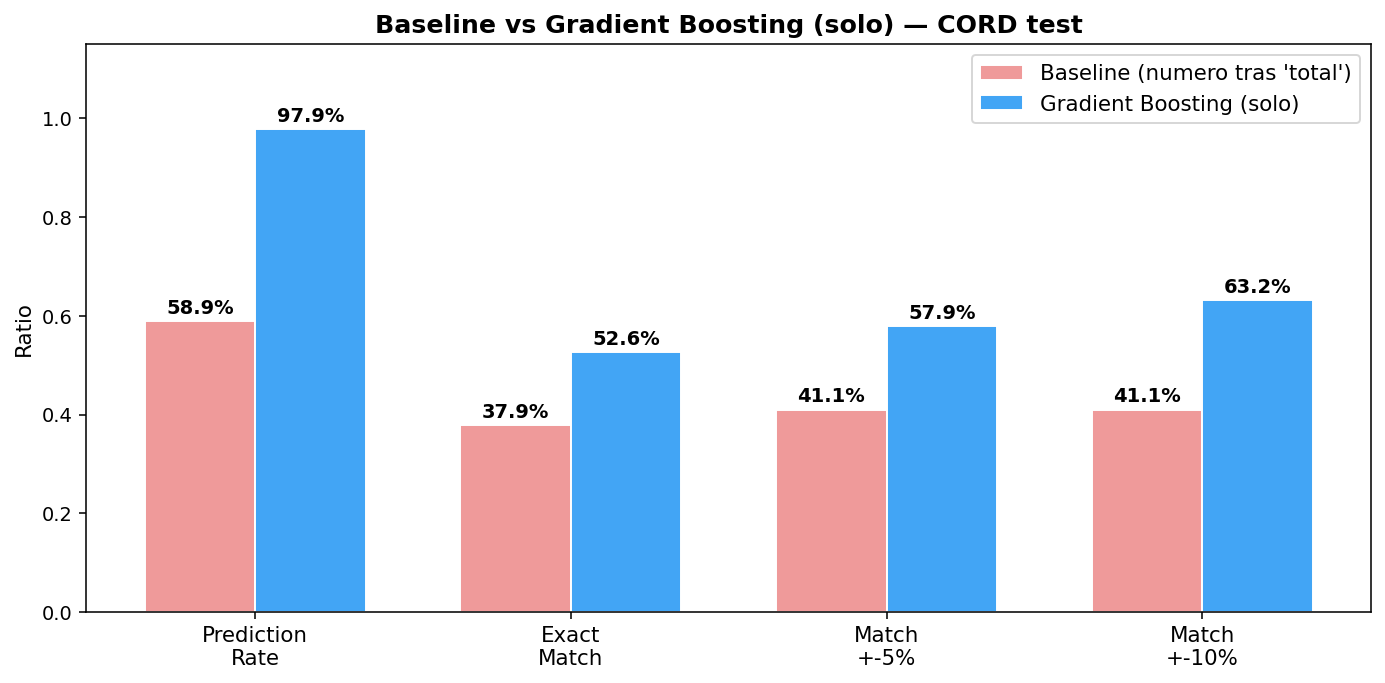
\includegraphics[width=0.8\textwidth]{figures/baseline_vs_gb.png}
    \caption{Baseline (número tras ``total'') vs Gradient Boosting usado como método principal: GB supera al baseline en todas las métricas}
    \label{fig:baseline_vs_gb}
\end{figure}

Sin embargo, Regex siempre devuelve un resultado (tiene fallback al número máximo), por lo que GB nunca se ejecutaba como fallback. La comparativa directa (Figura~\ref{fig:baseline_vs_gb}) confirmó que GB supera al baseline en +14,7~pp de Exact Match. \textbf{Decisión}: usar Gradient Boosting como método principal, no como fallback.

\subsection{Fase 3: Cambio de OCR --- PaddleOCR vs EasyOCR}

El análisis de tiempos reveló que el 99,95\% del tiempo se consumía en el OCR ($\sim$4,7~s con EasyOCR). Se evaluó PaddleOCR como alternativa.

\begin{figure}[t]
    \centering
    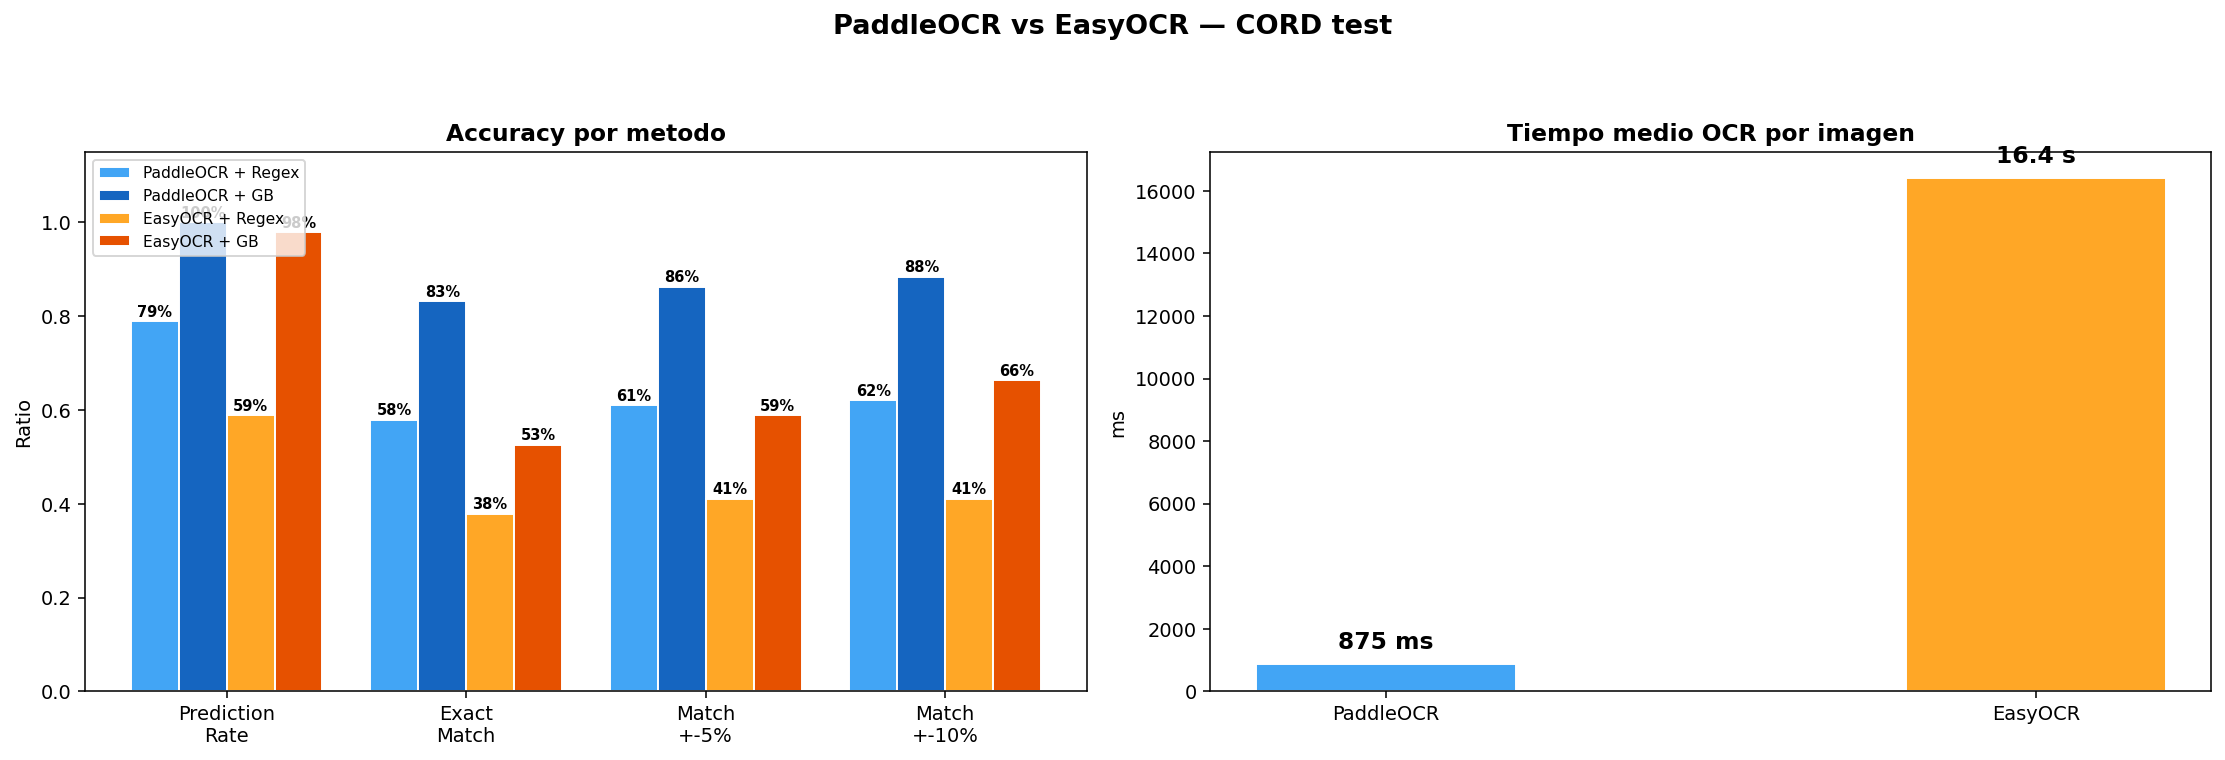
\includegraphics[width=\textwidth]{figures/paddleocr_vs_easyocr.png}
    \caption{Comparativa PaddleOCR vs EasyOCR sobre CORD test: PaddleOCR es 18,8$\times$ más rápido y aporta +30~pp en Exact Match}
    \label{fig:paddleocr_vs_easyocr}
\end{figure}

Como muestra la Figura~\ref{fig:paddleocr_vs_easyocr}, PaddleOCR resultó ser \textbf{18,8$\times$ más rápido} (875~ms vs 16.417~ms por imagen) y produjo texto de mucha mejor calidad, lo que se tradujo en +30 puntos porcentuales de Exact Match. PaddleOCR v2.8.1 con PaddlePaddle 2.6.2 fue la combinación estable utilizada, requiriendo Python 3.12.

\subsection{Pipeline final de producción}

El pipeline final integra los hallazgos de las tres fases:

\begin{enumerate}
    \item \textbf{PaddleOCR v2.8} --- Detección y reconocimiento de texto sobre la imagen ($\sim$875~ms).
    \item \textbf{Preprocesamiento de texto} --- Corrección de errores típicos de OCR ($\sim$0,2~ms).
    \item \textbf{Extracción de candidatos} --- Identificación de todos los números en el texto mediante expresiones regulares.
    \item \textbf{Feature engineering} --- Cálculo de 12 características por candidato: posición relativa en el documento, magnitud del número, proximidad a palabras clave (\textit{total}, \textit{amount}), contexto positivo y negativo, entre otras.
    \item \textbf{Gradient Boosting} --- Clasificador con 150 árboles y profundidad 5 que puntúa cada candidato y selecciona el de mayor probabilidad ($\sim$2~ms).
\end{enumerate}

\begin{table}[t]
    \centering
    \caption{Métricas finales del pipeline PaddleOCR + Gradient Boosting sobre 95 muestras de test CORD}
    \label{tab:metricas_finales}
    \begin{tabular}{lr}
        \toprule
        \textbf{Métrica} & \textbf{Valor} \\
        \midrule
        Exact Match & 83,2\% \\
        Match $\pm$5\% & 86,3\% \\
        Match $\pm$10\% & 88,4\% \\
        Prediction Rate & 100\% \\
        MRE & 0,12 \\
        Tiempo total/imagen & $\sim$877~ms \\
        Tamaño modelo GB & $\sim$2~MB \\
        Tamaño total pipeline & $\sim$350~MB \\
        \bottomrule
    \end{tabular}
\end{table}

Las métricas finales del pipeline se recogen en la Tabla~\ref{tab:metricas_finales}. El sistema alcanza un 83,2\% de coincidencia exacta con una cobertura del 100\% y un tiempo de procesamiento inferior a un segundo por imagen.

El sistema ofrece tres modos de uso: imagen individual (\texttt{-{}-image}), procesamiento por lotes de un directorio (\texttt{-{}-dir}) y captura en vivo con la cámara del dispositivo (\texttt{-{}-camera}).
